%%%%%%%%%%%%%%%%%%%%%%%%%%%%%%%%%%%%%%%%%%%%%%
%                insertmeeting
% 1) Title (something creative & funny?)
% 2) Date (MM/DD/YYYY)
% 3) Location (ex. Hagerty High School)
% 4) People/Committees Present 
% 5) Picture 
% 6) Start Time & Stop Time (ex. 12:30AM to 4:30PM)
%%%%%%%%%%%%%%%%%%%%%%%%%%%%%%%%%%%%%%%%%%%%%%
\insertmeeting 
	{Meeting Example} 
	{10/18/21} 
	{Hagerty High School}
	{Jensen}
	{Images/RobotPics/robot.jpg}
	{2:30 - 4:30}
	
\hhscommittee{Hardware}
\noindent\hfil\rule{\textwidth}{.4pt}\hfil
\subsubsection*{Goals}
\begin{itemize}
    \item Re evaluate drivetrain design 

\end{itemize} 

\noindent\hfil\rule{\textwidth}{.4pt}\hfil

\subsubsection*{Accomplishments}
After printing at ucf this weekend, we finally got to see the new 3d printed drivetrain (Figure \ref{fig:101821_1})! Upon seeing it, the first thing we noticed was that it seemed really big compared to what we had in mind. Because we were so surprised at its scale, we measured it to see if there had been a printing error, but we found that it was exactly as we had designed it. It seems that while we were CADing it, we lost our sense of scale, a common problem we have observed in the past, but that we have never experienced to this extent. As we looked over the design, we continued to notice features we had forgotten to add like pocketing holes that would make the drivetrain lighter and standoff holes that would hold metal standoffs, strengthening the drivetrain. We decided that some of the issues were too detrimental to simply leave alone, so we started redesigning. 
Although we could go through and make lots of small adjustments in the current drivetrain’s CAD document, there were so many errors that it made sense to just redesign from the ground up. Although we are keeping most of the design similar, we felt that redesigning would give us an opportunity to optimize the CAD, making it easier for us to change in the future. A large part of what we changed was just using more variables to control the significant dimensions of the design, like the thickness of the plastic, the length and width of the robot and the rib thickness (Figure \ref{fig:101821_2}). This will allow us to quickly make changes to the entire design by changing only one number. For instance, if we found that using a thickness of 1/8 inch for all of the surfaces of the design used too much material and was too heavy, we could change the variable for thickness (named depth in cad) to .1 inches, and the entire design would change. Knowing where we were going with the design also allowed us to make it more efficiently, as we knew key dimensions and what aspects of the design should be dependent upon them. We also made sure to fix all of the issues with the old design, like adding pocketing holes and stand-off holes. While designing, we made sure to keep a ruler nearby to help us understand the size that the robot was actually going to be. By doing this, we realized we could reduce both the length and the width of the drivetrain by 1.5 inches. Although we can't use the first version of the drivetrain we printed, it still helped us understand some of the physical properties of a 3d printed drivetrain of this scale, like the weight and strength. By testing these aspects of the first version, we found that the drivetrain was fairly light, but needed more support between the inner and outer drive plates, where we plan to add standoffs. One thing we noticed that was good about this first design is the ribs, which hold the inner drive plates very sturdily to the rest of the drivetrain.
One of the final features that we added was a curved lip at the corners of the drivetrain where we can wrap carbon fiber (Figure \ref{fig:101821_3}). Because we are unsure of how much damage the 3d printed drivetrain can withstand, we are thinking about getting carbon fiber and putting it over the top of the drivetrain. We added the lip because it is difficult to properly wrap carbon fiber over a 90 degree angle and the lip provides a smooth and gradual curve for it to rest over without compromising the structural integrity of the robot, as we would be doing if we just rounded the corners. After completing this, we believe we are finished with the cad for this iteration of the design (Figure \ref{fig:101821_4}), but want to get some other members to check it before printing. Part of the reason the first version had so many errors is that the same members who did most of the cad for it were the ones checking for errors. If we have someone look at the design with fresh eyes, they will hopefully catch all of our errors.

 

\begin{figure}[ht]
\centering
\begin{minipage}[b]{.48\textwidth}
  \centering
  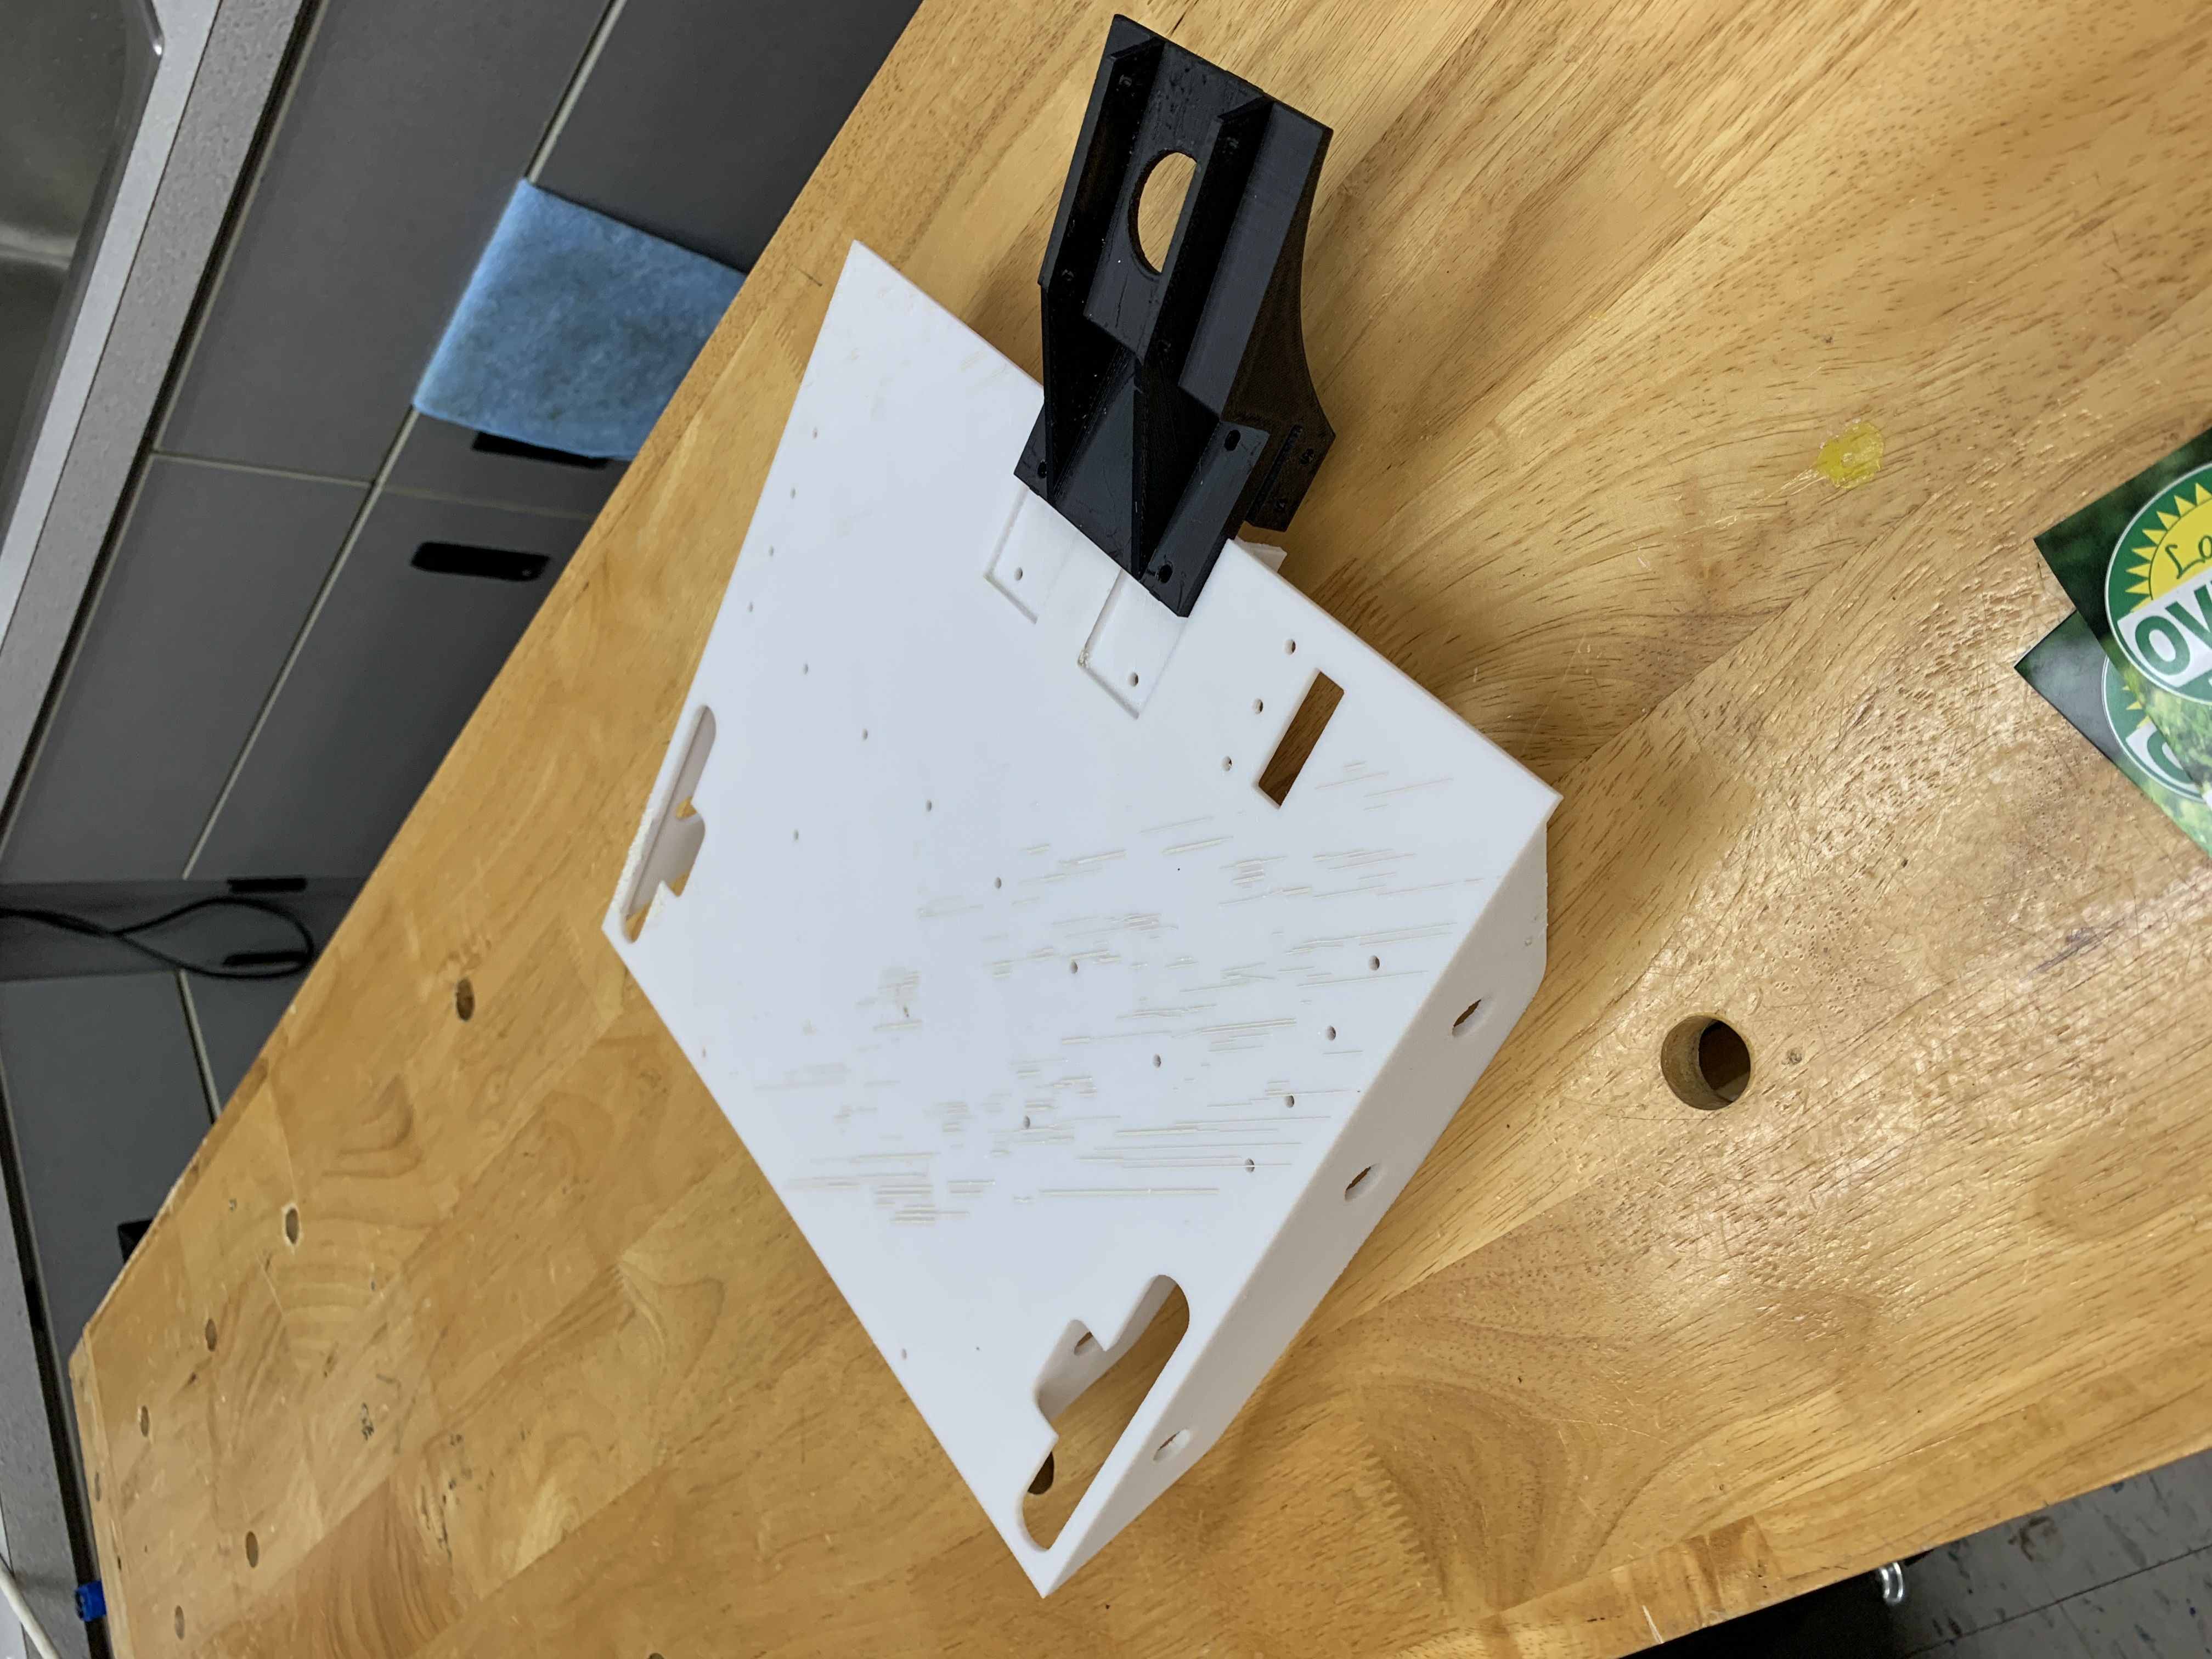
\includegraphics[width=0.95\textwidth]{Meetings/October/10-18-21/10-18-21_CAD_Figure1 - Nathan Forrer.JPG}
  \caption{The new 3D printed drivetrain}
  \label{fig:101821_1}
\end{minipage}%
\hfill%
\begin{minipage}[b]{.48\textwidth}
  \centering
  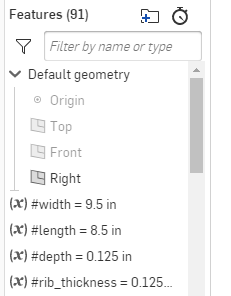
\includegraphics[width=0.95\textwidth]{Meetings/October/10-18-21/10-18-21_CAD_Figure2 - Nathan Forrer.PNG}
  \caption{Added CAD variables}
  \label{fig:101821_2}
\end{minipage}
\end{figure}


\begin{figure}[ht]
\centering
\begin{minipage}[b]{.48\textwidth}
  \centering
  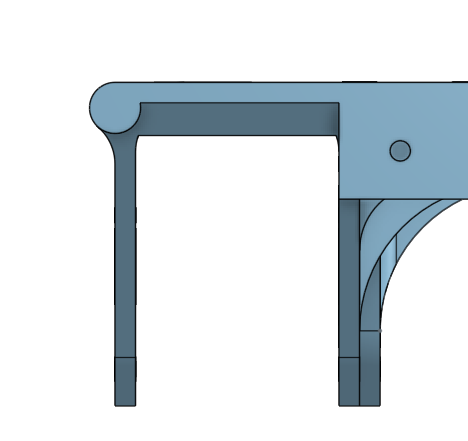
\includegraphics[width=0.95\textwidth]{Meetings/October/10-18-21/10-18-21_CAD_Figure3 - Nathan Forrer.PNG}
  \caption{Curved lip for carbon fiber}
  \label{fig:101821_3}
\end{minipage}%
\hfill%
\begin{minipage}[b]{.48\textwidth}
  \centering
  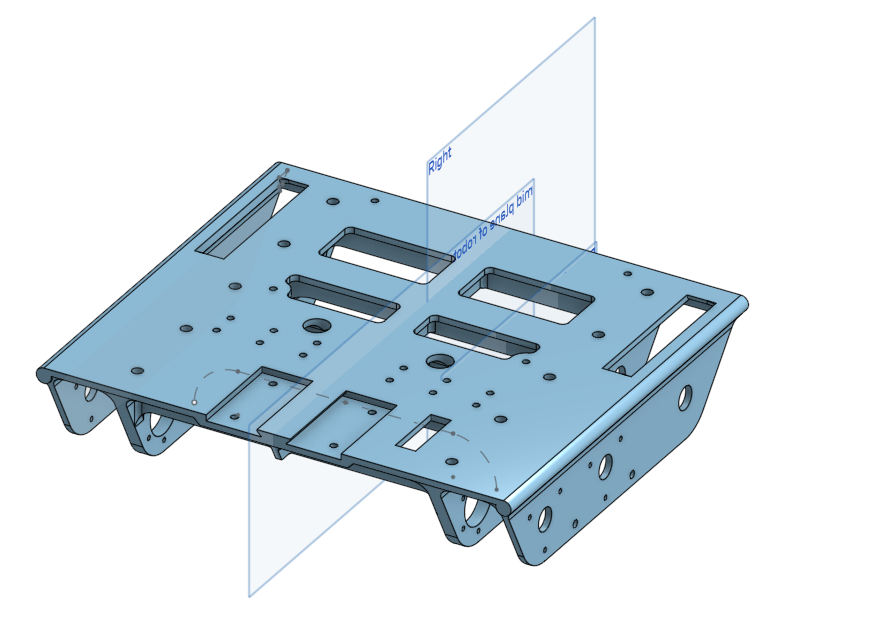
\includegraphics[width=0.95\textwidth]{Meetings/October/10-18-21/10-18-21_CAD_Figure4 - Nathan Forrer.PNG}
  \caption{Our current CAD iteration}
  \label{fig:101821_4}
\end{minipage}
\end{figure}



\whatsnext{
\begin{itemize}
    \item Check drivetrain v2 with other members
    \item Print drivetrain v2

\end{itemize} 
}

